% !TeX root = main.tex
\chapter{Technological developments}\label{app:tech}

\section{Dialogger}\label{sec:dialogger}

\texttt{https://github.com/bbc/dialogger}

\begin{figure}[h]
\centering
  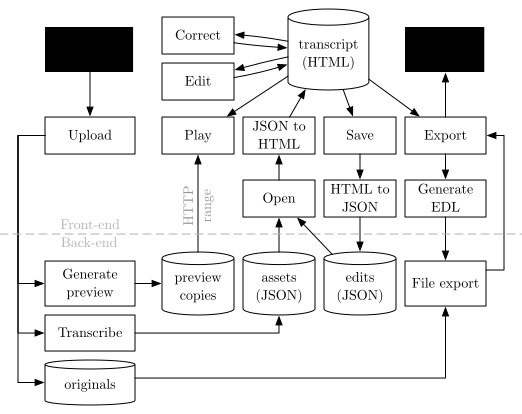
\includegraphics[width=\columnwidth]{figs/dialogger-flow-diagram.png}
  \caption{Flow diagram of the Dialogger system. Excluded components are shown in red.}
  \label{fig:dialogger-flow}
\end{figure}

Made a screen-based semantic speech editor. Here's how it works.

\clearpage
\section{Vampeyer}\label{sec:vampeyer}
The direction of the research in this project centres around turning audio data into image data. There is already some
software that visualizes audio and audio features in a number of ways, notably Sonic Visualiser \citep{Cannam2010}.
However, the visualization algorithms are always hard-coded into the program, making prototyping of new methods
prohibitively difficult.

\subsection{Design}
A system of software was developed for visualizing audio in order to allow flexibility while maintaining consist inputs
and outputs. It was designed to expand on existing systems for audio analysis so to avoid duplication of effort and to
allow modularisation of algorithms.

The system was developed as a plugin framework with clearly defined inputs and outputs. It is based on the existing
Vamp plugin framework, developed by Queen Mary University of London \citep{Cannam2010}, which analyses audio data and
outputs frame-- or time-based features. The visualization plugin is designed to take these features and produce a
bitmap image. An outline of the system design is shown in Figure~\ref{fig:vampeyer}.

\begin{figure}[ht]
  \centering
  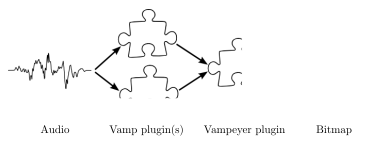
\includegraphics[width=0.8\textwidth]{figs/vampeyer.png}
  \caption{High-level system diagram of the Vampeyer visualization framework}
  \label{fig:vampeyer}
\end{figure}

The visualization plugin defines which Vamp plugin outputs it requires, including the block/step size and parameters.
At least one Vamp plugin is required, but there is no restriction of the number of different Vamp plugins that can be
used.

Both frameworks are written in C++ which allows for a fast processing time.  This is important for situations where
audio has to be processed on-the-fly, such as for exploring an archive without having to pre-process everything in it.
The plugins are compiled into shared libraries, so they can easily be distributed without users having to recompile
locally and integrated into third-party software.

\subsection{Implementation}
A C++ header file was created which implements the design.  Five data structures are also defined which define how data
should be sent and returned from the functions.

{\singlespacing
\begin{itemize}
  \item \texttt{VampParameter} is a name/value pair used to store a parameter
  \item \texttt{VampParameterList} is a vector of \texttt{VampParameter}s
  \item \texttt{VampPlugin} stores the name of a Vamp plugin along with a\\
    \texttt{VampParameterList} and the preferred block and step sizes
  \item \texttt{VampOutput} stores a \texttt{VampPlugin} and output name
  \item \texttt{VampOutputList} is a vector of \texttt{VampOutput}s
\end{itemize}
}

Two primary functions are used to define the input audio features and their conversion to a bitmap.

\begin{itemize}
  \item \texttt{getVampPlugins} returns a \texttt{VampOutputList} variable that contains a list of Vamp plugin outputs
    which must be provided as input
  \item \texttt{ARGB} takes the Vamp plugin output data as a \texttt{Vamp::FeatureSet} variable, the sample rate of the
    audio and the desired width and height. It returns a bitmap image formatted in 32-bit ARGB format (alpha, red,
    green, blue).
\end{itemize}

A number of example plugins were written to demonstrate the capabilities of this approach, and to act as useful pieces
of software in their own right.  These include a standard waveform, waveform colourised by low energy ratio (see
Section~\ref{sec:studywaveform}), waveform colourised by spectral centroid (identical to Freesound) and an MFCC grid
visualization with waveform overlay.

The plugins need to be run by a host program which reads the audio data, processes it using the Vamp plugins, sends
their output to the visualization plugin and then writes the image data. Such a program was written as a command-line
tool that can either display the image in a window or write it to disk as a PNG-encoded file. This makes it useful for
both prototyping and for back-end processing on a server, for example.

\clearpage
\section{BeatMap}\label{sec:beatmap}

